\label{Bijlage 1}

\appendix
\section{Bijlage 1: Versie Systeembeheer GIT}

\subsection*{Installatie en gebruik}\ \\

Bij gebruik van Git bash doen we ook beroep op msygit. Na de installatie van het programma gebruiken we de "Git Bash"\ en de volgende twee commando's om ons te kunnen identificeren. Dat zal later zijn nut bewijzen.\\
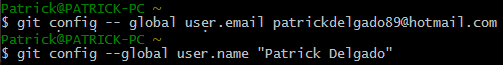
\includegraphics[width=0.7\textwidth]{git1.png}\\


Vervolgens moet er een SSH Key gegenereerd worden. Die zal zorgen voor de connectie tussen de documenten op de pc van de gebruiker en de online repository.\\

Voor het maken van deze sleutel wordt volgend commando gedaan.\\
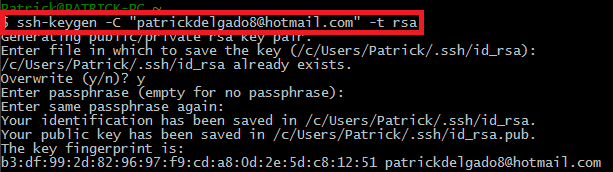
\includegraphics[width=0.7\textwidth]{git2.png}\\

Dat zal een folder .ssh aanmaken in de User Directory met de bestanden (id-rsa en id-rsa.pub). Het .pub bestand zullen we later nodig hebben voor de online repository server.\\

In de Windows Explorer rechtermuisklikken we op de map die we willen linken aan de online repository en kiezen we "Git Bash Here". Dat zal de Git Bash rechtstreeks openen met de link naar deze map en dan geven we het commando "git init"\ in. Dat vormt de map in een git repository om. In de map zelf wordt ook de map .git aangemaakt (normaal als verborgen). Als die verwijderd wordt zal de hoofdmap niet langer als een Git repository gezien worden.\\

Met het commando "git status"\ krijgen we een lijst van alle nieuwe, aangepaste of verwijderde bestanden te zien, die nog niet doorgevoerd zijn naar de online repository (deze is momenteel nog niet aangemaakt maar hier wordt later op teruggekomen).\\
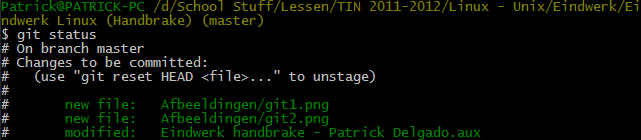
\includegraphics[width=0.7\textwidth]{git3.png}\\

Om de volledige map met al zijn bestanden voor te bereiden op verplaatsing naar de online repository, voeren we het commando "Git add ."\ uit.\\
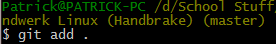
\includegraphics[width=0.5\textwidth]{git4.png}\\

Als we nu het commando "git status"\ ingeven, wordt er een lijst met alle veranderingen die zullen gebeuren weergegeven. Hierna wordt het commando "git commit -m \textless bericht\textgreater "\ gedaan om deze veranderingen klaar te zetten om door te sturen . Dat is een soort van toestemming geven aan het systeem om later deze wijzigingen door te voeren.\\
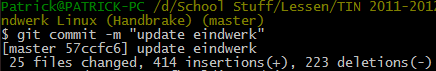
\includegraphics[width=0.7\textwidth]{git5.png}\\

Om verder te kunnen moeten we een repository maken. Op de site "www.github.com"\ kan men zich registreren voor een gratis account en opslagruimte. Na het aanmaken van een account moet de SSH key toegevoegd worden om de link te kunnen leggen van online opslag naar computer. Hiervoor gebruiken we het id-rsa.pub bestand. Open deze met notepad en kopieer de volledige inhoud. Bij de accountinstellingen is een gedeelte "SSH-Key"\ en dat voegen we hier toe.\\

Nu is het tijd om een repository te maken. Dat wordt gewoon gedaan op de Github hoofdpagina van de gebruiker via de knop "New repository". Verder hebben we volgende link nodig om verder te kunnen.\\
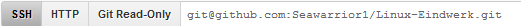
\includegraphics[width=0.7\textwidth]{git6.png}\\

Terug in de Git Bash gebruiken we volgend commando om de repository nu volledig te linken aan ons systeem.\\
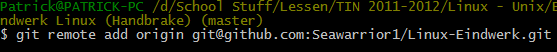
\includegraphics[width=1\textwidth]{git7.png}\\

Nu kunnen de bestanden naar de repository ge"upload worden met het commando "git push origin master". Alle bestanden die in de eerdere commit stonden worden nu gepushed naar de server voor online opslag.\\
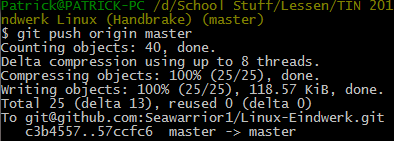
\includegraphics[width=0.7\textwidth]{git8.png}\\

Om bestanden te verwijderen wordt gebruik gemaakt van het commando "git rm naambestand"\. Om deze wijziging dan door te voeren worden gewoon de commando's "git commit -m 'boodschap'"\ en "git push origin master" gebruikt.\\
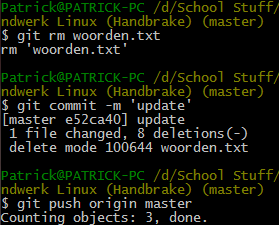
\includegraphics[width=0.5\textwidth]{git9.png}\\
\pagebreak


